\documentclass[12pt, a4paper]{article}

\usepackage[portuguese]{babel}
\usepackage[utf8]{inputenc}
\usepackage[a4paper,top=2.54cm,bottom=2.0cm,left=2.54cm,right=2.54cm]{geometry}
\usepackage[bottom]{footmisc}
\usepackage{graphicx}
\usepackage{listings}
\usepackage{minted}

\author{Victor Alberto Romero}
\title{Como ativar as bandeiras de compilação}

\begin{document}
\maketitle

No curso explica-se que a forma usada para compilar arquivos fonte que vai ser usada é a seguinte:

\begin{minted}{bash}
  > gcc -Wall -ansi -O2 -pedantic arquivo.c -o exec
\end{minted}

Esta forma de compilação inclui algumas opções que são passadas ao compilador duma forma conhecida em programação como bandeiras. Estas bandeiras vão pedir ao compilador ter algumas considerações especiais na hora de fazer seu trabalho. O objetivo de essas bandeiras específicas no curso é ajudar ao estudante a detetar erros potenciais de programação, mostrando para ele coisas que podem estar certas, mas que \textit{parecem} que não estejam.

Mas para as pessoas que trabalham em Dev-C++ não é muito evidente como passar este conjunto de opções. Para isso foi criado este mini tutorial. O objetivo então é habilitar quatro bandeiras (flags) na compilação, estas são:

\begin{itemize}
  \item Wall: É uma abreviação de \textit{Warning all}. Faz que todas as alertas sejam mostradas na hora de compilar.
  \item ansi: Habilita compatibilidade com o padrão ansi.
  \item O2: Opções de otimização nível dois.
  \item pedantic: Faz o compilador mais estrito com os padrões de código.
\end{itemize}

As bandeiras podem ser ligadas nas opções de compilação de Dev-C++. A continuação mostram-se algumas capturas de tela indicando exatamente em que lugar estão estas opções. Para as capturas foi usada a versão estável mais recente do aplicativo encontrada na hora de gerar este tutorial, que é Dev-C++ 5.7.1\footnote{http://sourceforge.net/projects/orwelldevcpp/}.

\section*{Ativação das bandeiras}

Para ativar as bandeiras vai se ao menu \emph{Ferramentas}, submenu \emph{Opções do Compilador}, como pode-se ver na Figura~\ref{fig:1}.

\begin{figure}[H]
  \centering
  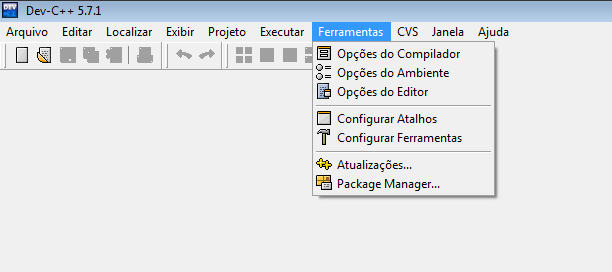
\includegraphics[width=140mm]{Imagens/1.png}
  \caption{Menu de Ferramentas}
\label{fig:1}
\end{figure}

Na nova ventana que aparece, na aba \emph{Configurações}, sub-aba \emph{Opções C} ativa-se a opção \emph{Suporte a todos os padrões ANSI (-ansi)}, como da para ver na Figura~\ref{fig:2}.

\begin{figure}[H]
  \centering
  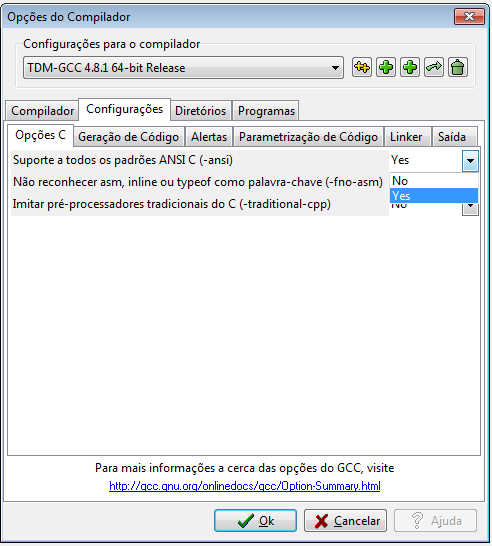
\includegraphics[width=90mm]{Imagens/2.png}
  \caption{Opção ansi}
\label{fig:2}
\end{figure}

Depois na sub-aba \emph{Geração de Código} modifica-se a opção \emph{Nível de otimização (-Ox)} a \emph{High} (o que é equivalente à bandeira O2), como pode-se ver na Figura~\ref{fig:3}.

\begin{figure}[H]
  \centering
  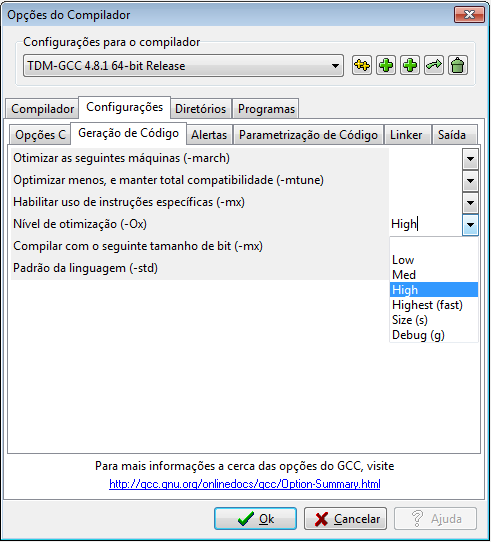
\includegraphics[width=90mm]{Imagens/3.png}
  \caption{Opção O2}
\label{fig:3}
\end{figure}

Por último, na sub-aba \emph{Alertas} ativam-se as opções \emph{Exibir maioria dos alertas (-Wall)} e \emph{Verificar conformação com ISO C/C++/C++0x (-pedantic)}, como pode-se ver na Figura~\ref{fig:4}. 

\begin{figure}[H]
  \centering
  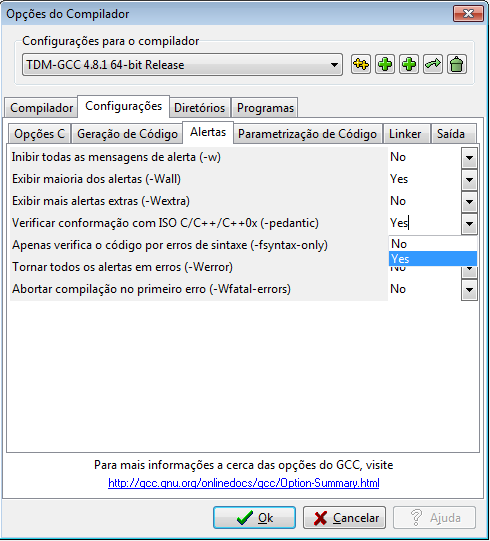
\includegraphics[width=90mm]{Imagens/4.png}
  \caption{Opções Wall e pedantic}
\label{fig:4}
\end{figure}

Com isso fica pronto, a compilaão agora vai conter todas as bandeiras usadas no curso.

\end{document}
